\documentclass[11pt]{article}
\usepackage{spikey}
\usepackage[margin=1in]{geometry}

\usepackage{physics}
\usepackage{amsmath}
\usepackage{tikz}
\usepackage{mathdots}
\usepackage{yhmath}
\usepackage{cancel}
\usepackage{color}
\usepackage{siunitx}
\usepackage{array}
\usepackage{multirow}
\usepackage{amssymb}
\usepackage{gensymb}
\usepackage{tabularx}
\usepackage{booktabs}
\usetikzlibrary{fadings}
\usetikzlibrary{patterns}
\usetikzlibrary{shadows.blur}
\usetikzlibrary{shapes}

\title{Inverse Propensity Score Weighting}
\author{Tianyu Du}

\begin{document}
\maketitle
\paragraph{} Let $X, Y, Z$ denote the cause, the effect, and confounding variables. Let $\mc{X}, \mc{Y}, \mc{Z}$ denote domains of above-mentioned random variables. Let $f(Y)$ denote the random variable of interest. Then,
\begin{align}
	\expe[f(Y)|do(X=x)] &= \sum_{y \in \mc{Y}, z \in \mc{Z}} f(y) P(X=x,Y=y,Z=z|do(X=x)) \\
	&= \sum_{y \in \mc{Y}, z \in \mc{Z}} f(y) P(Y=y|X=x, Z=z) P(Z=z) \\
	&= \sum_{y \in \mc{Y}, z \in \mc{Z}} f(y) \frac{P(X=x, Y=y | Z=z)}{P(X=x|Z=z)} P(Z=z) \\
	&=\sum_{y \in \mc{Y}, z \in \mc{Z}} f(y) \frac{P(X=x, Y=y, Z=z)}{P(X=x|Z=z)}
\end{align}
	where $P(X=x|Z=z)$ is the \textbf{propensity score}, which denotes the probability of receiving treatment $X=x$ given characteristics $Z=z$.
	
	Assume there is a finite dataset of size $N$, $(x_i, y_i, z_i)_{i=1}^N$, and we wish to infer the interventional distribution of $f(Y)$ using this dataset.

	One method used for discrete variables is to simply count the occurrence of each $(X, Y, Z)$ in the dataset.
\begin{align}
	\hat{P}(X=x, Y=y, Z=z) &= \frac{\sum_{i=1}^N \id{x_i=x} \id{y_i=y} \id{z_i=z}}{N}
\end{align}
	Therefore,
\begin{align}
	\hat{\expe}[f(Y)|do(X=x)] &= \sum_{y \in \mc{Y}, z \in \mc{Z}} \frac{f(y)}{P(X=x|Z=z)} \frac{\sum_{i=1}^N \id{x_i=x} \id{y_i=y} \id{z_i=z}}{N} \\
	&= \frac{1}{N} \sum_{i=1}^N \frac{f(y_i)}{P(X=x_i|Z=z_i)} \label{1}
\end{align}
	The estimation (\ref{1}) is the inverse-propensity-score weighted mean of $f(y_i)$.
\begin{figure}
\caption{The Causal Graph}
\medbreak
\centering
\tikzset{every picture/.style={line width=0.75pt}} %set default line width to 0.75pt        

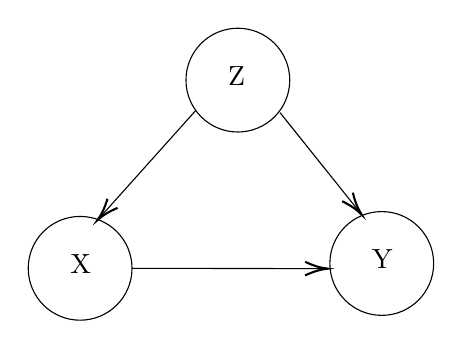
\begin{tikzpicture}[x=0.75pt,y=0.75pt,yscale=-1,xscale=1]
%uncomment if require: \path (0,300); %set diagram left start at 0, and has height of 300

%Shape: Circle [id:dp03511134286032647] 
\draw   (100,146) .. controls (100,132.19) and (111.19,121) .. (125,121) .. controls (138.81,121) and (150,132.19) .. (150,146) .. controls (150,159.81) and (138.81,171) .. (125,171) .. controls (111.19,171) and (100,159.81) .. (100,146) -- cycle ;
%Shape: Circle [id:dp7665684229342842] 
\draw   (245.33,143.67) .. controls (245.33,129.86) and (256.53,118.67) .. (270.33,118.67) .. controls (284.14,118.67) and (295.33,129.86) .. (295.33,143.67) .. controls (295.33,157.47) and (284.14,168.67) .. (270.33,168.67) .. controls (256.53,168.67) and (245.33,157.47) .. (245.33,143.67) -- cycle ;
%Shape: Circle [id:dp15774530961848976] 
\draw   (176,55.33) .. controls (176,41.53) and (187.19,30.33) .. (201,30.33) .. controls (214.81,30.33) and (226,41.53) .. (226,55.33) .. controls (226,69.14) and (214.81,80.33) .. (201,80.33) .. controls (187.19,80.33) and (176,69.14) .. (176,55.33) -- cycle ;
%Straight Lines [id:da4142747561916664] 
\draw    (221.33,71) -- (259.42,118.6) ;
\draw [shift={(260.67,120.17)}, rotate = 231.34] [color={rgb, 255:red, 0; green, 0; blue, 0 }  ][line width=0.75]    (10.93,-3.29) .. controls (6.95,-1.4) and (3.31,-0.3) .. (0,0) .. controls (3.31,0.3) and (6.95,1.4) .. (10.93,3.29)   ;
%Straight Lines [id:da1397091872063163] 
\draw    (180.67,70) -- (134.67,121.34) ;
\draw [shift={(133.33,122.83)}, rotate = 311.86] [color={rgb, 255:red, 0; green, 0; blue, 0 }  ][line width=0.75]    (10.93,-3.29) .. controls (6.95,-1.4) and (3.31,-0.3) .. (0,0) .. controls (3.31,0.3) and (6.95,1.4) .. (10.93,3.29)   ;
%Straight Lines [id:da7004401912765537] 
\draw    (150,146) -- (242.33,146.16) ;
\draw [shift={(244.33,146.17)}, rotate = 180.1] [color={rgb, 255:red, 0; green, 0; blue, 0 }  ][line width=0.75]    (10.93,-3.29) .. controls (6.95,-1.4) and (3.31,-0.3) .. (0,0) .. controls (3.31,0.3) and (6.95,1.4) .. (10.93,3.29)   ;

% Text Node
\draw (119,138) node [anchor=north west][inner sep=0.75pt]   [align=left] {X};
% Text Node
\draw (264.33,135.67) node [anchor=north west][inner sep=0.75pt]   [align=left] {Y};
% Text Node
\draw (195,47.33) node [anchor=north west][inner sep=0.75pt]   [align=left] {Z};
\end{tikzpicture}
\end{figure}
\end{document}
